\subsection{SQL版の概要}

  \if0
  特定の病気にかかっている複数人の患者の医療情報が記載された
  エクセルファイルを医療関係者から提供していただいた.
  医療情報として検査値,投薬についての情報などが記載されていた.
 このエクセルのデータのみを受け付けるWebアプリケーション
  をDjangoで開発した.

  検査値,投薬についての情報を患者の認可のもとで収集し,
  SQLデータベースに保存する.
  患者に認可をされた医療関係者は情報の参照,書き込みが可能となる.

  このサービスを実現するために後述する機能を実装した.

  本研究ではユーザとして患者と医療関係者の2つの立場があることを
  想定している.
  ユーザモデルは二者を区別できるように実装し,
  二者で異なる使い方ができるようにした.
  \fi


  鈴鹿医療科学大学からある病気にかかっている患者の検査値と
  投薬に関する情報が記載されたエクセルファイルを提供していただいた.
  これをサンプルとして用いて医療情報を共有することができる
  Webアプリケーションを開発した.
  電子カルテや医療情報共有ソフトを導入できない医療機関でも
  患者の医療情報を共有できるようにすることが目的である.

  \begin{figure}[htbp]
    \begin{center}
      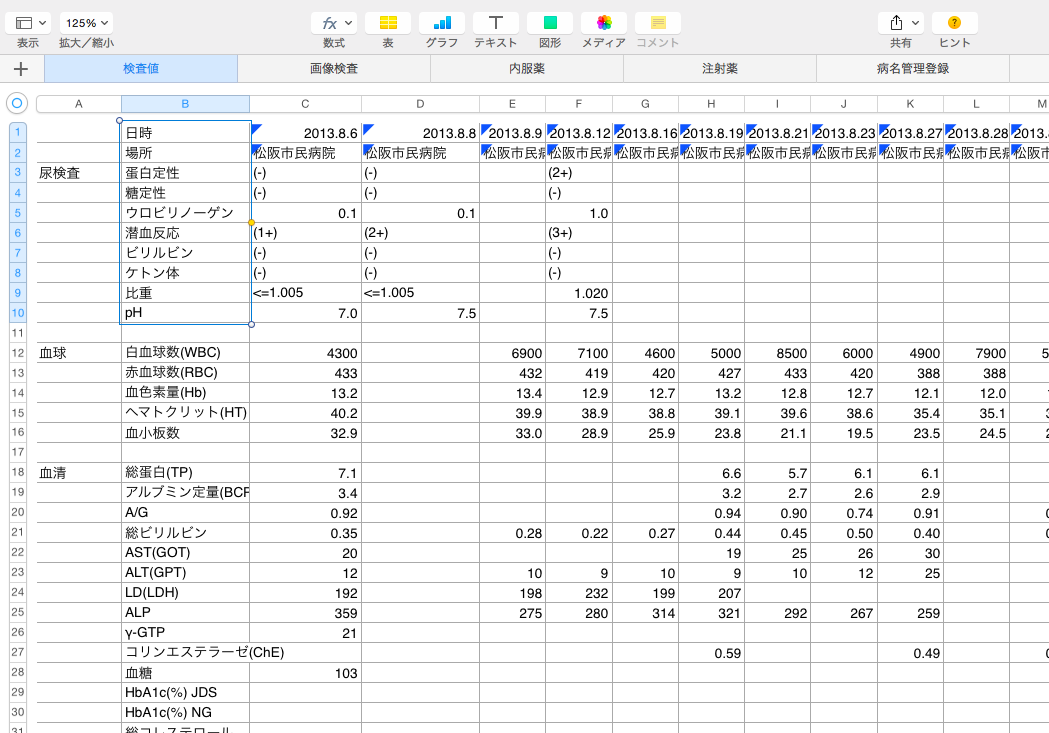
\includegraphics[width=10cm, bb=0 0 1049 733]{./gazou/excel-data.png}
    \end{center}
    \caption{エクセルファイルの例}
    \label{excel-data}
  \end{figure}

  \begin{figure}[htbp]
    \begin{center}
      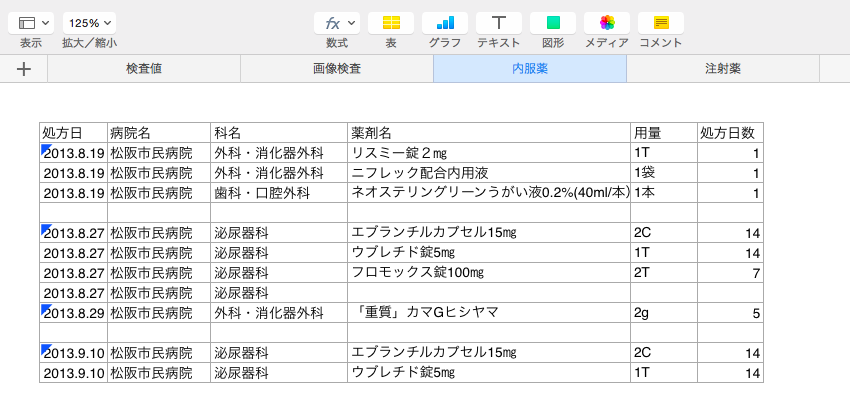
\includegraphics[width=10cm, bb=0 0 850 411]{./gazou/excel-data-medicine.png}
    \end{center}
    \caption{内服薬のエクセルファイルの例}
    \label{excel-data-medicine}
  \end{figure}


\subsection{想定する利用方法}
   患者によって閲覧,書き込みが許可された医療関係者は,
  他の医療関係者によって入力された医療情報を
  Webインターフェース上で閲覧することができる.
  また,患者と他の医療関係者が閲覧できるように
  検査,診断などによって得られた
  新たな医療情報を追記することができる.

   患者はWebインターフェースにより自身の医療情報の
  閲覧をすることができるので,
  図\ref{DjangoTable}の表で検査値の推移を確認できる.
  また,図\ref{DjangoGantt}の
  ガントチャートによって処方すべき治療薬の種類,期間,数量を
  確認することができる.

  さらに,医療情報共有システムを導入していない医療機関に
  かかるときは患者の端末で自身の医療情報を提示することで
  医療情報共有システムの恩恵を与えることができる.
  %医療関係者に既往歴を閲覧させることができる.


\subsection{設計}
  システムのユースケース図とクラス図は
  図\ref{system_construct},
  図\ref{class}のようになっている.
  医療関係者は患者の医療情報の閲覧と書き込みの機能を利用する際,
  患者から認可が出ていることが必要となる.
  患者は医療機関係者に認可を出す権限を持っている.

  \begin{figure}[htbp]
    \begin{center}
      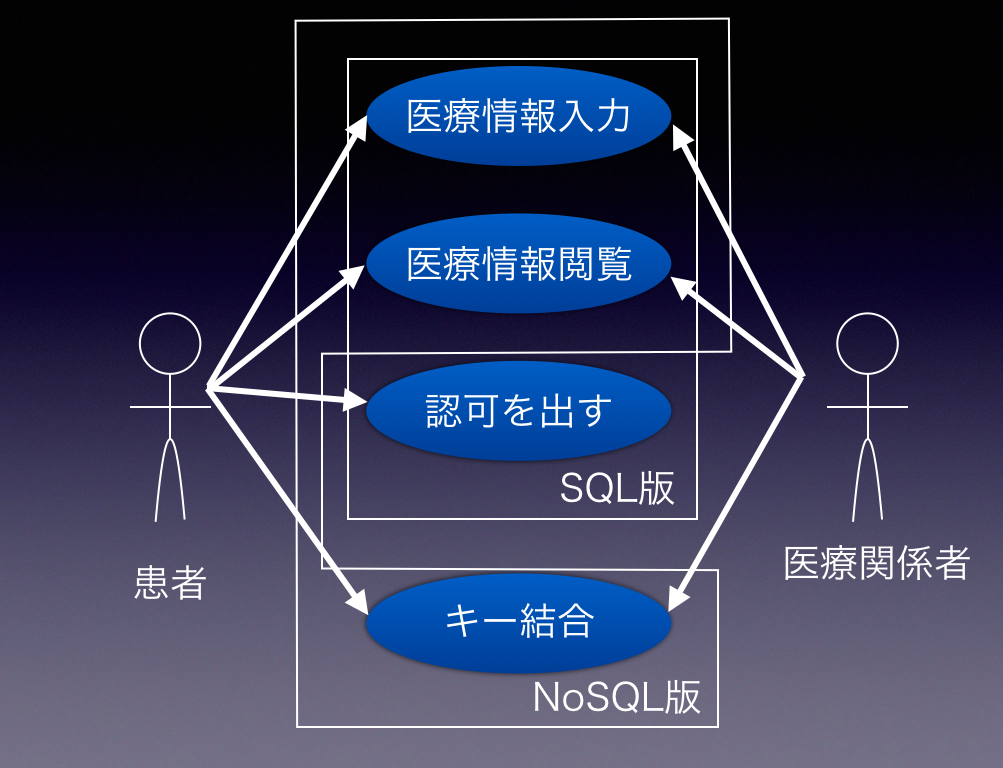
\includegraphics[width=10cm, bb=0 0 1003 768]{./gazou/system_construct2.png}
    \end{center}
    \caption{システムのUMLユースケース図}
    \label{system_construct}
  \end{figure}

  \begin{figure}[htbp]
    \begin{center}
      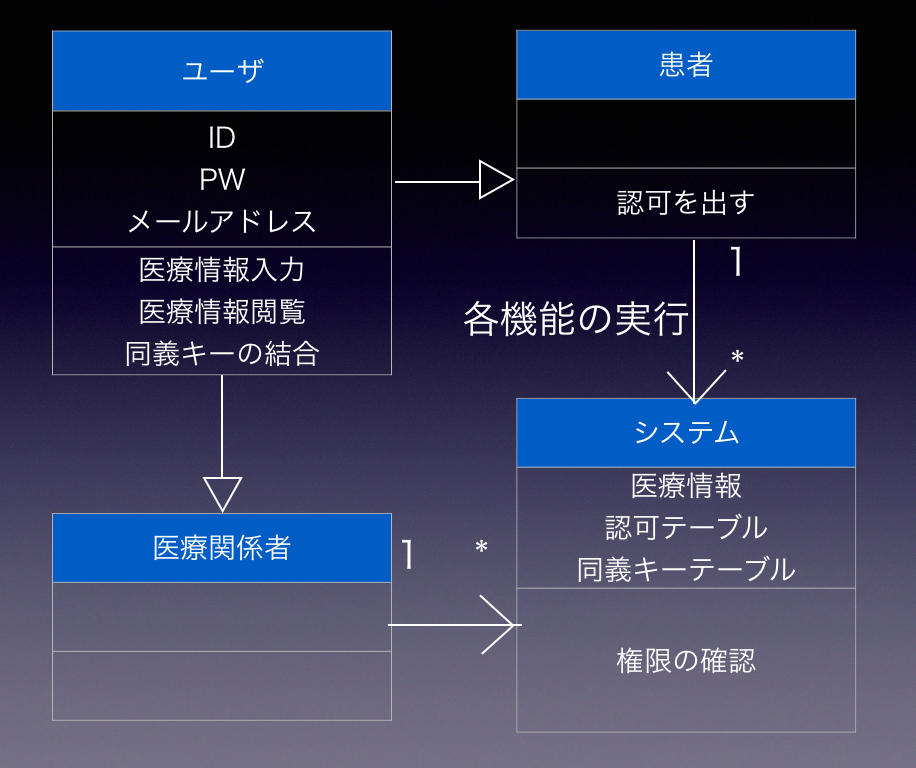
\includegraphics[width=10cm, bb=0 0 916 760]{./gazou/class.png}
    \end{center}
    \caption{UMLクラス図}
    \label{class}
  \end{figure}

\subsection{機能}
  \subsubsection{権限の付与}
    患者の医療情報をどの医療関係者が操作することができるかを
    患者自身が選択する.
    認可には段階を設けた.
    具体的には,閲覧不可,閲覧可能と書き込み可能の
    3段階の認可を用意することである.
    これにより,医療関係者は患者の意志を尊重しながら
    医療情報を活用することができる.


  \subsubsection{データ入力}
    データベースには提供していただいたエクセルファイルの記述方法に対応する
    SQLのテーブルを用意している.
    ファイルをアプリケーションが図\ref{DjangoFileio}の
    ページで受け取ると検査値と投薬についての
    情報を医療情報をデータベースへ入力することができる.

  \subsubsection{データ閲覧}
    診断データは表にして、縦方向に診断項目,
    横方向に診断を行った日をとっている.
    空白部分はデータが入力されていない項目である.
    (図\ref{DjangoTable})


    投薬データはある薬をどれだけの期間服用しているかを
    わかりやすくするためにガントチャートのように表示している.
    色によってカテゴリの視認性を向上させたため,
    複数の医療機関にかかっている際に発生する可能性がある
    同時に服用することが好ましくない薬の組み合わせや
    過度な投薬を医療関係者が発見しやすい.(図\ref{DjangoGantt})



    \begin{figure}[htbp]
      \begin{center}
        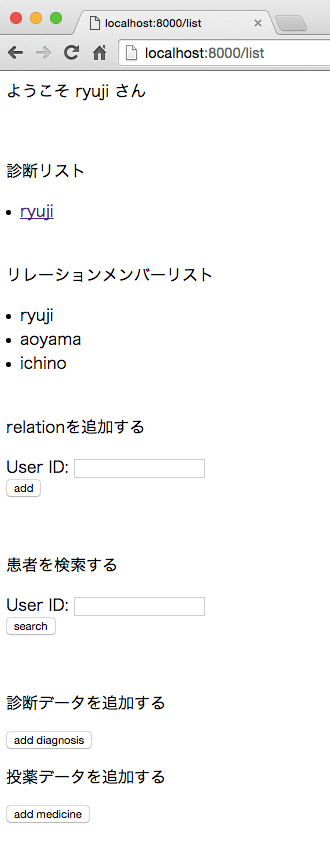
\includegraphics[width=7cm, bb=0 0 330 851, clip]{./gazou/DjangoFileio2.png}
      \end{center}
      \caption{データ入力画面}
      \label{DjangoFileio}
    \end{figure}

    \begin{figure}[htbp]
        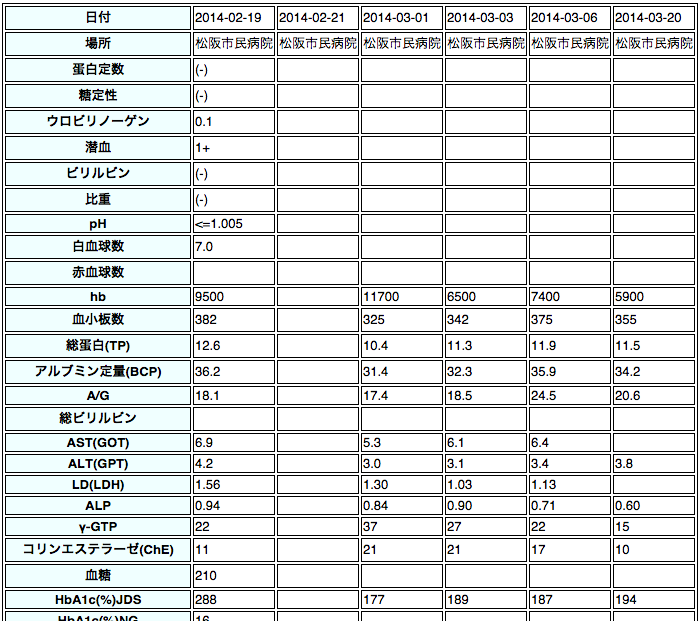
\includegraphics[width=15cm, bb=0 0 698 621]{./gazou/DjangoTable2.png}
      \caption{表によるデータ閲覧}
      \label{DjangoTable}
    \end{figure}

    \begin{figure}[htbp]
        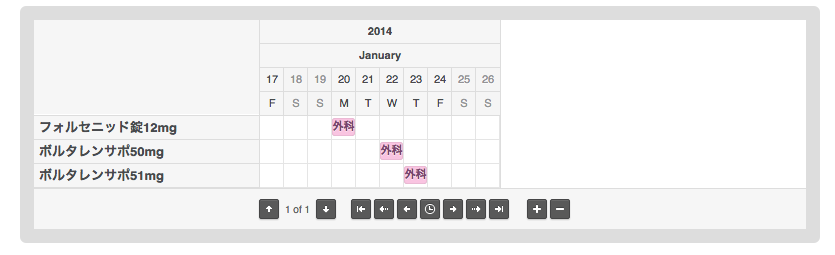
\includegraphics[width=15cm, bb=0 0 835 221]{./gazou/DjangoGantt2.png}
      \caption{ガントチャートによるデータ閲覧}
      \label{DjangoGantt}
    \end{figure}



\subsection{SQL版のまとめ}
  医療機関に依存していないので,
  病院ごとの患者IDなどを取得する必要はない.
  ユーザに独自のアカウントを割り当てて
  医療情報共有Webアプリを利用させる.

  認可を患者が出す

  入力形式がエクセルファイルに限定される.
  しかも項目の内容制限がある.


  \if0

  開発アプリのデモンストレーションをデータを提供していただいた
  医療関係者に対して行った.
  そのときにいただいたWebアプリケーション改善のための意見の中で
  研究課題として任意の検査項目の抽出が挙げられる.

  他の意見はインターフェース寄りの要望が多かった.
  例えば,表によるデータの表示に対するフィードバックとして,
  任意の検査項目にハイライトをつけてほしいといった内容であったが,
  本研究で工数を割くことができなかったため開発を見送った.


  ドキュメントの数だけSQLデータベースのテーブルを用意する必要がある.
  データを検索する際にはjoinしてから.
  比べてNoSQLならガンガン入れて,
  データを出すときにだけKeyの関連づけをすればよい.
  NoSQLならSQLに比べてテーブルを用意する分の
  コストがはぶけてる(と言えるかな).
  \fi
